
Multiple testing problems are a staple of modern data-driven studies, where a large number of hypotheses are formulated and screened for their plausibility simultaneously.
This multiplicity of tests brings along a multitude of challenges, and have been a subject of extensive study in recent years.
% in the literature of high-dimensional statistics.


We are motivated in particular by the high-dimensional variable screening problems for categorical data. 
A prototypical example is genome-wide association studies (GWAS), where a large number of categorical genetic factors are examined for their impact on the phenotypic traits.
These categorical covariate screening problems naturally give rise to the high-dimensional chi-square models, introduced through the language of GWAS next.

\subsection{Genome-wide association studies and the chi-square model}
\label{subsec:motivation-chisq}

Broadly speaking, GWAS aim to discover genetic variations that are linked to traits or diseases of interested, by testing for associations between the subjects' genetic compositions and their phenotypes \citep{bush2012genome}.
In a typical GWAS with case-control design, a total of $n$ subjects are recruited consisting of $n_1$ subjects possessing the defined trait, and $n_2$ subjects without the trait.
The genetic compositions of these subjects are then sequenced for variations known as single-nucleotide polymorphisms (SNPs) at an array of $p$ genomic marker locations, and compared between the case group and the control group.

Focusing on one specific genomic location, the counts of observed genotypes, if two variants are present, can be tabulated as follows.
\begin{center}
    \begin{tabular}{cccc}
    \hline
    & \multicolumn{2}{c}{Genotype} & \\
    \cline{2-3}
    \# Observations & Variant 1 & Variant 2 & Total by phenotype \\
    \hline
    Cases & $O_{11}$ & $O_{12}$ & $n_1$ \\
    Controls & $O_{21}$ & $O_{22}$ & $n_2$ \\
    \hline
    \end{tabular}
\end{center}
Statistical tests are then performed on the tabulated counts to detect associations.
A common test of association is Pearson's Chi-square test, with statistic
\begin{equation} \label{eq:chisq-statistic}
    x = \sum_{j=1}^2 \sum_{k=1}^2 \frac{(O_{jk} - E_{jk})^2}{E_{jk}},
\end{equation}
where $E_{jk}$'s are the expected number of observations in respective cells, estimated empirically with $E_{jk} = (O_{j1}+O_{j2})(O_{1k}+O_{2k})/n$.
%E_{jk} = \Big(\sum_{l}O_{jl}\Big)\Big(\sum_{l}O_{lk}\Big)\Big/n.

Under the mild assumption that the counts $O_{jk}$'s follow a multinomial distribution, the statistic $x$ in \eqref{eq:chisq-statistic} can be shown to have an approximate $\chi^2(\lambda)$ distribution with $\nu=1$ degree of freedom at large sample sizes \citep{agresti2018introduction}. 
When genotypes and phenotypes are independent, the non-centrality parameter $\lambda$ is identically zero; and if dependence exists, we have $\lambda\neq0$ where its value depends on the underlying multinomial probabilities.
More generally, if we have a $J$ phenotypes and $K$ genetic variants, assuming a $J\times K$ multinomial distribution, the statistic will follow approximately a $\chi^2_{\nu}(\lambda)$ distribution with $\nu = (J-1)(K-1)$ degrees of freedom, when sample sizes are large.

The same asymptotic distributional approximations are also applies to the likelihood ratio statistic, and many other statistics under slightly different modeling assumptions \cite{gao2019upass}.
These association tests are performed at each of the $p$ SNP marker locations throughout the whole genome, yielding $p$ statistics having approximately (non-)central $\chi^2_{\nu}$ distributions,
\begin{equation} \label{eq:model-chisquare-approx}
    x(i) \mathrel{\dot\sim} \chi_{\nu(i)}^2\left(\lambda(i)\right), \quad i=1,\ldots,p,
\end{equation}
where $\lambda = (\lambda(i))_{i=1}^p$ is the $p$-dimensional non-centrality parameter.
%, with $\lambda(i)=0$ indicating independence of the $i$-th SNP with the outcomes, and $\lambda(i)\neq0$ indicating associations.

With the number of genomic locations $p$ in genetic association studies usually in the order of $10^5$ or even $10^6$, it is often believed that only a small set of genetic variants have large influences on the outcome of the disease or trait of interest .
Under the stylized assumption of exact sparsity, $\lambda$ is assumed to have $s$ non-zero components, where $s$ is much smaller than the problem dimension $p$. 
The goal of researchers is two-fold: 1) to test if $\lambda(i)=0$ for all $i$, and 2) to estimate the set $S=\{i:\lambda(i)\neq 0\}$.
In other words, we look to determine if there are any genetic variation associated with the disease; and if there are associations, we wish to locate the associated variants.

The latter, referred to as the \emph{support recovery problem}, is the focus of this work.
We will study in detail the theoretical limits in support recovery problems in an idealized model where the statistics follow independent
% \footnote{In practice, dependence among the genetic markers at different locations (known as linkage disequilibrium) decay rapidly as a function of their physical distances on the genome, the correlations of the resulting statistics are roughly independent except at short distances.}
chi-square distributions,
\begin{equation} \label{eq:model-chisq}
    %x(i) \distras{\mathrm{ind.}} \chi_\nu^2\left(\lambda(i)\right), \quad i=1,\ldots,p.
    x(i) \sim \chi_\nu^2\left(\lambda(i)\right), \quad i=1,\ldots,p.
\end{equation}
We will also look for practical procedures that attain the performance limits, as soon as the problems become theoretically feasible.


\subsection{Two-sided alternatives of additive error models}
\label{subsec:motivation-additive}

The chi-square model \eqref{eq:model-chisq} arise in problems much more general than association screenings.
In particular, it plays an important role in analyzing variable screening problems with omnidirectional tests.
An important example is multiple two-sided tests in additive error models,
\begin{equation} \label{eq:model-additive}
    x(i) = \mu(i) + \epsilon(i), \quad i=1,\ldots,p,
\end{equation}
where the errors $\epsilon$ are assumed to have standard normal distributions.

Under two-sided alternatives, unbiased tests call for rejecting the hypothesis $\mu(i)=0$ at locations where observations have large absolute values, or equivalently, large $x^2(i)$'s.
Taking squares on both sides of \eqref{eq:model-additive}, and we arrive at Model \eqref{eq:model-chisq} with non-centrality parameters $\lambda(i) = \mu^2(i)$ and degrees-of-freedom parameter $\nu =1$.
In this case, the support recovery problem becomes to locate the set of observations with mean shifts, $S=\{i:\mu(i)\neq 0\}$, where the mean shifts could take place in both directions.

While theoretical limits of support recovery problems in additive error models \eqref{eq:model-additive} have been extensively studied (see, e.g., \cite{arias2017distribution, butucea2018variable, gao2018fundamental}), such studies were focused exclusively on one-sided alternatives.
On the other hand, in many applications, restricting ourselves to one-sided alternatives is insufficient.
For example, in fMRI studies, average brain activities at each of the tens of thousands of voxels may be either higher or lower in the case group compared to the controls \citep{narayan2015two}. 
In the challenging application of anomaly detection on Internet traffic streams, millions of IP addresses need to be scanned in real time to identify both volumetric attacks and blackouts \citep{kallitsis2016amon}.
In general, both the locations and the directions of the signals are unknown, and many interesting results obtained under one-sided alternatives unfortunately do not apply.

Studying model \eqref{eq:model-chisq} will allow us to tackle the omnidirectional alternatives, which are arguably more realistic in discovery sciences where little to no prior knowledge is available.
In comparing with results on one-sided alternatives in the additive model \eqref{eq:model-additive}, we will also be able to quantify if, and how much of a price has to be paid for the additional uncertainty of the two-sided alternatives .

\subsection{Contributions}

The contribution of this work is three-fold.

First, we show that several common family-wise error rate controlling procedures, including Bonferroni's procedure \cite{dunn1961multiple}, are asymptotically optimal to first order for \emph{exact} support recovery problems in the chi-square model \eqref{eq:model-chisq}.
Second, we show that the Benjamini-Hochberg (BH) procedure \cite{benjamini1995controlling} is asymptotically optimal to first order for \emph{approximate} support recovery problems.

These two results, under appropriate parametrizations of the signal sizes and sparsity levels in $\lambda$, establish the phase transitions of support recovery problems in the chi-square model.
They previewed in Figure \ref{fig:phase-chi-squared}, and made precise in Theorems \ref{thm:chi-squred-strong-boundary} and \ref{thm:chi-squred-weak-boundary}.
The results also reveal that the exact support recovery problems in the additive models can be substantially harder under the two-sided alternatives compared to the one-sided case, while the approximate support recovery problems are not.
Remarkably, the degree-of-freedom parameter does not affect the asymptotic boundaries in both problems.


\begin{figure}
      \centering
      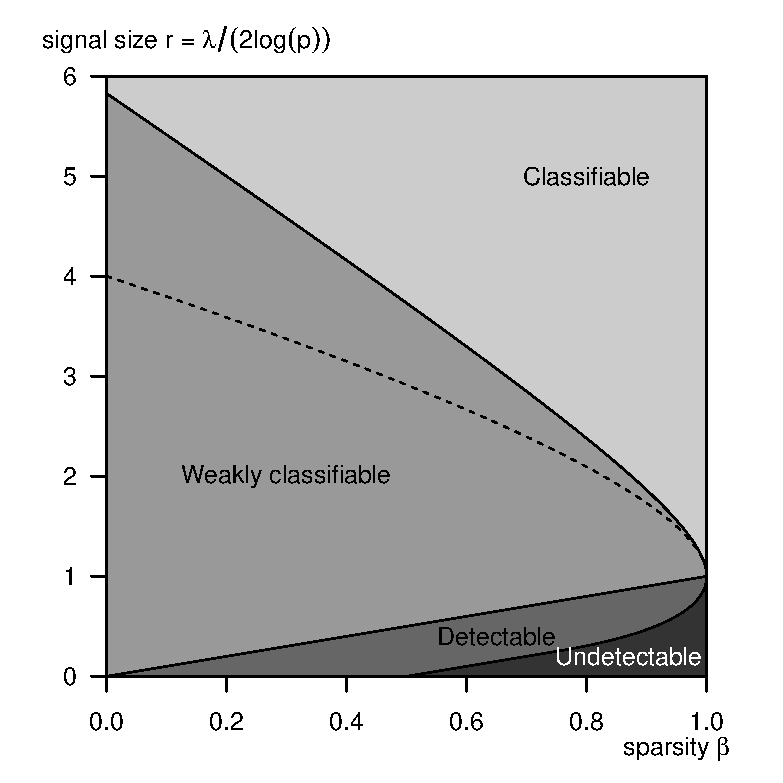
\includegraphics[width=0.7\textwidth]{./phase_diagram_chisquared.eps}
      % 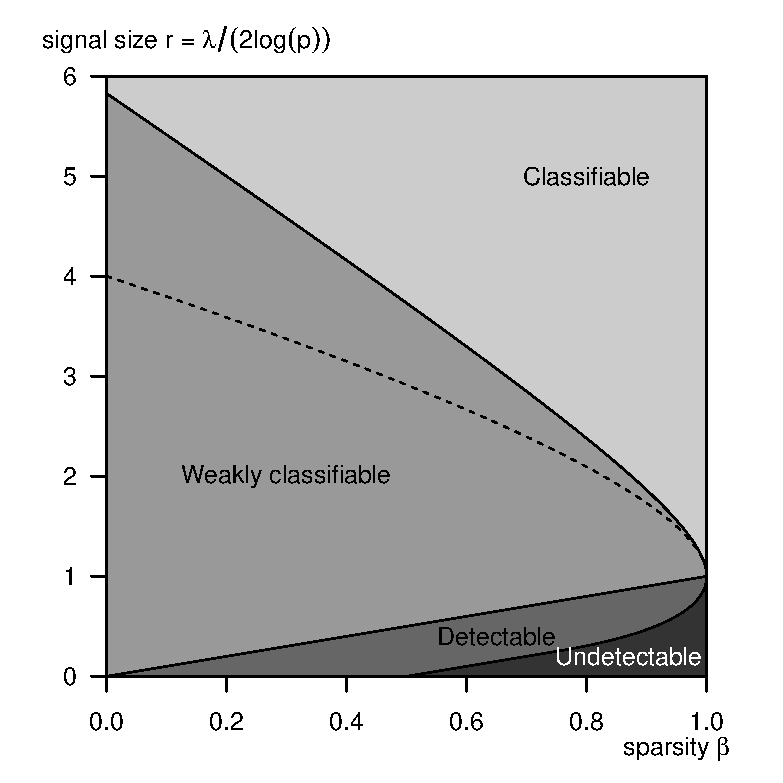
\includegraphics[width=0.35\textwidth]{./phase_diagram_chisquared.eps}
      \caption{The phase diagram of the high-dimensional chi-square model \eqref{eq:model-chisq}, illustrating the boundaries of the exact (Theorem \ref{thm:chi-squred-strong-boundary}) and approximate support recovery problems (Theorem \ref{thm:chi-squred-weak-boundary}), and the signal detection problem (described in \citep{donoho2004higher}). 
      The risk of exact support recovery \eqref{eq:risk-exact} can be made to vanish above the strong classification boundary \eqref{eq:strong-classification-boundary-chisquared} in the \emph{classifiable} region with, e.g., Bonferroni's procedure; conversely, the risk has liminf at least one.
      Similarly, the risk of approximate support recovery \eqref{eq:risk-approximate} can be made to vanish above the weak classification boundary \eqref{eq:weak-classification-boundary-chisquared} in the \emph{weakly classifiable} region with Benjamini-Hochberg's procedure; conversely, the risk has liminf at least one.
      Both boundaries are unaffected by the degrees-of-freedom parameter in the model.
      In comparison, the strong classification boundary for one-side alternatives in the additive model \eqref{eq:model-additive} under Gaussian noise (dashed line) is substantially lower than in the chi-square model; the weak classification and detection boundaries are identical to that in chi-square models.} 
      \label{fig:phase-chi-squared}
\end{figure}


Unlike in additive error models, the notion of signal size in chi-square models is often not as transparent.
Our third contribution demystifies this notion in the context of association tests.
We do so by characterizing of the relationship between signal sizes and marginal frequencies, odds ratio, and sample sizes for association tests on 2-by-2 contingency tables.
% Specifically, the amount of signal, when rare variants are present, is weaker compared to the signal when the marginal distributions are balanced.
% In other words, reliable detection of the effects by rare variants would require more samples compared to common variants, even at the same odds ratio.
The relationship between sample sizes and signal sizes, is made quantitative in Proposition \ref{prop:signal-size-odds-ratio}.

Together, these results allows us to work out the signal sizes, and in turn, the sample sizes needed to achieve a desired accuracy of support recovery, from the problem dimensionality and assumed sparsity levels.

\subsection{Statistical risks in support recovery problems}
\label{subsec:risks}

Recall that in support recovery problems, our goal is to come up with a procedure, denoted $\mathcal R$, to produce a set estimate $\widehat{S}$ of the true index set of relevant variables  $S=\{i:\lambda(i)\neq 0\}$.
The set estimate depends on the procedure $\mathcal{R}$, which in turn, takes as input the data or test statistics $x$.
We suppress this dependence by writing $\widehat{S}$ in place of $\widehat{S}(\mathcal{R}(x))$ for notational convenience when it does not lead to ambiguity.

For a given procedure $\mathcal{R}$, the \emph{false discovery rate} (FDR) is defined to be the expected fraction of false findings not in the true index set, among the reported discoveries \cite{benjamini1995controlling}. That is,
\begin{equation} \label{eq:FDR}
    \mathrm{FDR}(\mathcal{R}) = \E\left[\frac{|\widehat{S}\setminus S|}{\max\{|\widehat{S}|,1\}}\right].
\end{equation}
Similarly, \emph{false non-discovery rate} (FNR), which measures the power of the procedure, is defined as the expected fraction of missed detections,
\begin{equation} \label{eq:FNR}
    \mathrm{FNR}(\mathcal{R}) = \E\left[\frac{|S\setminus \widehat{S}|}{\max\{|{S}|,1\}}\right].
\end{equation}
Following \cite{arias2017distribution, rabinovich2017optimal}, we define the risk for \emph{approximate} support recovery as
\begin{equation} \label{eq:risk-approximate}
    \mathrm{risk}^{\mathrm{A}}(\mathcal{R}) = \mathrm{FDR}(\mathcal{R}) + \mathrm{FNR}(\mathcal{R}).
\end{equation}

A more stringent criteria for false discovery in multiple testing problems is family-wise error rate (FWER), defined to be the probability of reporting at least one finding not contained in the true index set.
That is,
\begin{equation} \label{eq:FWER}
    \mathrm{FWER}(\mathcal{R}) = 1 - \P[\widehat{S} \subseteq S].
\end{equation}
Correspondingly, a more stringent criteria for false non-discovery is family-wise non-discovery rate (FWNR), defined as the probability of missing at least one finding in the true index set,
\begin{equation} \label{eq:FWNDR}
    \mathrm{FWNR}(\mathcal{R}) = 1 - \P[S \subseteq \widehat{S}].
\end{equation}
Analogous to the risk for approximate support recovery, we define the risk for \emph{exact} support recovery as
\begin{equation} \label{eq:risk-exact}
    \mathrm{risk}^{\mathrm{E}}(\mathcal{R}) = \mathrm{FWER}(\mathcal{R}) + \mathrm{FWNR}(\mathcal{R}).
\end{equation}
An intimately related measure of success in the exact support recovery problem is the probability of exact recovery 
\begin{equation} \label{eq:risk-prob}
    \P[\widehat{S} = S] = 1 - \P[\widehat{S} \neq S].
\end{equation}
The relationship between $\P[\widehat{S} = S]$ and $\mathrm{risk}^{\mathrm{E}}$ will be discussed in Section \ref{sec:chisq-boundaries}, where we study the performance of procedures in support recovery problems in terms of the risk metrics defined here.

\subsection{Thresholding procedures}
\label{subsec:thresholding-procedures}

We shall study the performance of five procedures in Section \ref{sec:chisq-boundaries}.
All of them belong to the broad class of thresholding procedures, defined as follows.
\begin{definition}[Thresholding procedures]
A thresholding procedure for estimating the support 
$S:=\{i\, :\, \lambda(i)\neq0\}$ is one that takes on the form
\begin{equation} \label{eq:thresholding-procedure}
    \widehat{S} = \left\{i\,|\,x(i) > t(x)\right\},
\end{equation}
where the threshold $t(x)$ may depend on the data $x$.
\end{definition}
Examples of thresholding procedures include ones that aim to control FWER -- Bonferroni's \cite{dunn1961multiple}, Sid\'ak's \citep{vsidak1967rectangular}, Holm's \citep{holm1979simple}, and Hochberg's procedure \citep{hochberg1988sharper} -- as well as ones that target FDR, such as Benjamini-Hochberg's procedure \cite{benjamini1995controlling} and Cand\'es-Barber's procedure \cite{barber2015controlling}.
Indeed, thresholding procedures \eqref{eq:thresholding-procedure} is such a general class that it contains most of the statistical procedures in the multiple testing literature \cite{roquain2011type}.

We shall restrict our discussion to the class of thresholding procedures.
Specifically, the lower bounds that we develop in Theorems \ref{thm:chi-squred-strong-boundary} and \ref{thm:chi-squred-weak-boundary} below are only meant to apply to such procedures.

\begin{remark}
While it is intuitively appealing to consider only threshold procedures, such procedures are not always optimal.
Recently, \citet{chen2018scan} showed that thresholding procedures are in fact sub-optimal in the additive models \eqref{eq:model-additive} when errors have heavy (regularly-varying) tails. 
\citet{gao2018fundamental} recently characterized the conditions under which thresholding procedures are optimal in exact support recovery problems.
The optimality of thresholding procedures in approximate support recovery problems is an open problem that invites a separate discussion. 
We content ourselves with making optimality statements concerning only thresholding procedures in the current work.
\end{remark}


\subsection{More related work}

Performance limits of statistical procedures in the additive error model \eqref{eq:model-additive} under one-sided alternatives is a well-studied topic.
For approximate support recovery, measured in terms of the risk of approximate support recovery \eqref{eq:risk-approximate}, \citet*{arias2017distribution} established the asymptotic optimality of the Benjamini-Hochberg procedure \cite{benjamini1995controlling}, and the Cand\'es-Barber procedure \cite{barber2015controlling} for independent additive errors;
\citet{rabinovich2017optimal} further established the rate-optimality of both procedures under the same regime.

When the goal is the more stringent exact support recovery, measured in terms of \eqref{eq:risk-exact}, it was recently shown in \cite{gao2018fundamental} that several well-known FWER-controlling procedures are optimal, even under severe dependence and general distributional assumptions.
Similar results were obtained in terms of the Hamming loss, for specific procedures in the additive models \cite{butucea2018variable} and in the regression context \cite{ji2012ups,jin2014optimality} under Gaussian errors.

The sparse signal detection problem in the high-dimensional chi-square model \eqref{eq:model-chisq} was studied in \cite{donoho2004higher},
while the support recovery problems remain unexplored.
\citet{sun2007oracle} studied general strategies of multiple testing problems, which includes the two-sided alternatives in the normal model as a major example; their proposed likelihood ratio thresholding procedure requires consistent estimation of the non-null distributions and the mixture proportions.

Asymptotic power approximations of association tests on contingency tables can be found in, e.g., \cite{ferguson2017course}, and many other texts on asymptotic statistics.
A companion paper to the current work \cite{gao2019upass} analyzed asymptotic equivalences of several additional common association tests, and implements the power calculations in a software tool for visualization and forensics of reported findings in genetic association studies.


